\documentclass{beamer}

\usepackage[backend=bibtex,maxnames=100]{biblatex} %from macports texlive-bibtex-extra
\addbibresource{refs.bib}
\renewcommand{\footnotesize}{\tiny}

\usepackage{listings}
\usepackage{xcolor}
\definecolor{verylightgray}{gray}{0.95}
\definecolor{somewhatdarkgray}{gray}{0.3}
\lstset{
  language=,
  basicstyle=\footnotesize\ttfamily,
  numberstyle=\tiny,
  numbersep=5pt,
  tabsize=2,
  extendedchars=true,
  breaklines=true,
  keywordstyle=\color{red},
  stringstyle=\color{blue}\ttfamily,
  numberstyle=\color{violet},
  showspaces=false,
  showtabs=false,
  showstringspaces=false,
  backgroundcolor=\color{verylightgray},
  frame=single,
  framexleftmargin= 3px,
  framexrightmargin= 3px,
  rulecolor=\color{lightgray}
}

% http://tex.stackexchange.com/questions/226929/making-algorithm2e-environments-overlay-aware-in-beamer
\resetcounteronoverlays{algocf}

\usetheme{Madrid}
\setbeamertemplate{navigation symbols}{} % Remove the navigation symbols
\setbeamertemplate{sections/subsections in toc}[default] %Turn off ugly toc numbering
\setbeamertemplate{itemize subitem}[triangle]
\setbeamertemplate{itemize item}[triangle]
\setbeamertemplate{enumerate items}[default]
%\setbeamercovered{transparent}
\usepackage{appendixnumberbeamer}
\defbeamertemplate{section page}{customsection}[1][]{%
  \begin{centering}
    {\usebeamerfont{section name}\usebeamercolor[fg]{section name}#1}
    \vskip1em\par
    \begin{beamercolorbox}[sep=12pt,center]{part title}
      \usebeamerfont{section title}\insertsection\par
    \end{beamercolorbox}
  \end{centering}
}
\defbeamertemplate{subsection page}{customsubsection}[1][]{%
  \begin{centering}
    {\usebeamerfont{subsection name}\usebeamercolor[fg]{subsection name}#1}
    \vskip1em\par
    \begin{beamercolorbox}[sep=8pt,center,#1]{part title}
      \usebeamerfont{subsection title}\insertsubsection\par
    \end{beamercolorbox}
  \end{centering}
}
\AtBeginSection{\frame{\sectionpage}}
%\AtBeginSubsection{\frame{\subsectionpage}}

%%%%%%%%%%%%%%%%%%%%%%%%%%%%%%%%%%%%%%%%%%%%%%%%%%%%%%%%%%%%%%%%%%%%%%%%%%%%%%%

\graphicspath{{./images/}}

% Customize hyperref here
% color links, but not internal links (confusing..)
\hypersetup{colorlinks=true,linkcolor=}

\usepackage{tikz}
\usepackage{algorithm}
\usepackage{nicefrac}
\usepackage[noend]{algpseudocode}
\usepackage{booktabs}
\algnewcommand{\Goto}[1]{\textbf{goto } #1}
\algnewcommand{\Break}{\textbf{break}}

\author[Patrick Sanan]{Patrick Sanan \\ \href{mailto:patrick.sanan@erdw.ethz.ch}{\texttt{patrick.sanan@erdw.ethz.ch}}}

%%%%%%%%%%%%%%%%%%%%%%%%%%%%%%%%%%%%%%%%%%%%%%%%%%%%%%%%%%%%%%%%%%%%%%%%%%%%%%%

\title[]{Short Valgrind Tutorial} 
\date[]{March 6, 2017} 
% Long date messes up footer

%%%%%%%%%%%%%%%%%%%%%%%%%%%%%%%%%%%%%%%%%%%%%%%%%%%%%%%%%%%%%%%%%%%%%%%%%%%%%%%

\begin{document}
\setbeamertemplate{section page}[customsection]
\setbeamertemplate{subsection page}[customsubsection]

%%%%%%%%%%%%%%%%%%%%%%%%%%%%%%%%%%%%%%%%%%%%%%%%%%%%%%%%%%%%%%%%%%%%%%%%%%%%%%%%
%%%%%%%%%%%%%%%%%%%%%%%%%%%%%%%%%%%%%%%%%%%%%%%%%%%%%%%%%%%%%%%%%%%%%%%%%%%%%%%%

\begin{frame}[fragile]
\titlepage 
\begin{center}
  This presentation (with examples): \url{https://bitbucket.org/psanan/valgrind_tutorial} \\
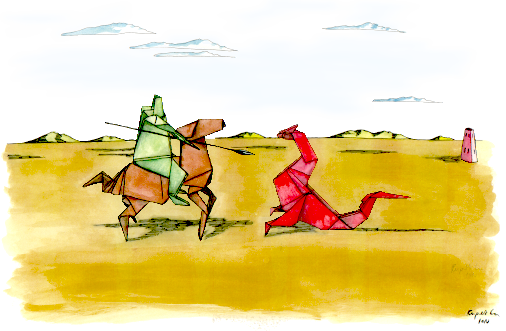
\includegraphics[height=0.25\textheight]{st-george-dragon.png}\\
{\tiny \url{http://valgrind.org/images/st-george-dragon.png}}
\end{center}
\end{frame}

\section{Introduction}

\begin{frame}[fragile]
\frametitle{What's in a name?}
\begin{itemize}
\item Valgrind, the gate to Valhalla \\
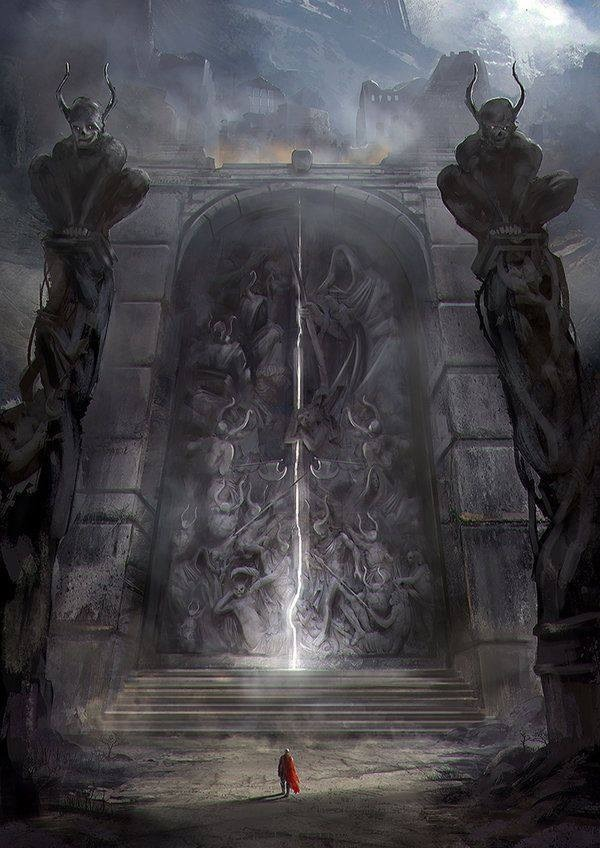
\includegraphics[height=0.3\textheight]{gate.jpg} 
\item Pronounced like ``Val grinned'' \\

\includegraphics[height=0.3\textheight]{val.jpg} 
\item \url{http://valgrind.org/docs/manual/faq.html#faq.pronounce}
\end{itemize}
\end{frame}

\begin{frame}[fragile]
\frametitle{What's the Problem?}
\begin{itemize}
\item In programming languages like C and Fortran, you are responsible for your own dynamic memory management
\item You reserve memory on the \emph{heap} with which to do your computations
\item You return this memory when you are finished with it
\item You are responsible for only accessing memory locations that you have reserved
\item You can make mistakes!
\begin{itemize}
\item Forgetting to return memory
\item Reading and writing into memory you haven't reserved
\item Using uninitialized memory to control logic
\end{itemize}
\item These are all {\bf unacceptably bad things to do}, but the compiler can't warn you*
\item Valgrind helps detect and locate these mistakes, using just your executable
\end{itemize}
\end{frame}

\section{Installation (aka the worst part)}

\begin{frame}[fragile]
\frametitle{Obtaining Valgrind}
\begin{itemize}
  \item Bad news: Valgrind does {\bf not} work on OS X 10.11 and 10.12 (it worked sporadically before that).
    \begin{itemize}
      \item MacPorts will install it for you, but it doesn't work!
    \end{itemize}
\item Valgrind works very well on most Linux systems, and is often available through a package manager
\begin{lstlisting}[language=bash]
sudo apt-get install valgrind
\end{lstlisting}
\item Valgrind is actually quite easy to download and build yourself (but probably still won't work on recent OS X systems) \\
  \url{http://valgrind.org/downloads/current.html}
\end{itemize}
\end{frame}

\begin{frame}[fragile]
  \frametitle{Building Valgrind 3.12.0 on Euler (thanks to Ilya Fomin)}
  \begin{itemize}
    \item Get the source onto Euler
      \begin{lstlisting}
    ssh euler
    wget http://valgrind.org/downloads/valgrind-3.12.0.tar.bz2
    tar xvf valgrind-3.12.0.tar.bz2
      \end{lstlisting}
\item configure, build, and install. It will take a long time.
  Don't move the binary from this location!
  \begin{lstlisting}
    cd valgrind-3.12.0
    mkdir -p $HOME/valgrind_install
    ./configure --prefix=$HOME/valgrind_install
    make && make install
  \end{lstlisting}
\item Add to your path
  \begin{lstlisting}
  export PATH=$PATH:$HOME/valgrind_install  # can go in your login file (e.g. .bashrc)
    which valgrind
  \end{lstlisting}
\item Make sure it runs (by testing the built in \texttt{ls -l} function)
  \begin{lstlisting}
    valgrind ls -l
    echo "valgrind ls -l" > tmp.sh && bsub < tmp.sh && rm tmp.sh  
      # examine resulting lsf.xxx 
  \end{lstlisting}
  \end{itemize}
\end{frame}

\section{Basic Usage}

\begin{frame}[fragile]
\frametitle{Using Valgrind}
\begin{itemize}
\item Valgrind is very easy to use; just supply your program, with arguments
\begin{lstlisting}
valgrind ./my_program -arg1 -arg2
valgrind -- ./my_program -arg1 -arg2 # sometimes required
\end{lstlisting}
\item It helps greatly to include debugging symbols (compile with \texttt{-g}\footnote{unless you care about executable size, you should also do this with optimized builds})
\item Output can be more meaningful if you compile without optimization, e.g. \texttt{-O0}.
\item You can redirect valgrind's output to a file with \texttt{--log-file}, for example
  \begin{lstlisting}
valgrind --log-file=valgrind.log ./my_program
  \end{lstlisting}
\item The combined program output and valgrinds output can be directed both the screen and to a file with standard UNIX tools:
  \begin{lstlisting}
valgrind ./my_program 2>&1 | tee valgrind_all.txt
  \end{lstlisting}
\end{itemize}
\end{frame}

\begin{frame}[fragile]
\frametitle{Hello, World}
\begin{itemize}
\item By default, valgrind uses the Memcheck tool, which checks for dynamic memory errors.
\item See \texttt{examples/1\_hello} (you need working gcc and/or gfortran compilers)
  \item I've provided most of the examples in C and fortran, but will mostly refer to the C versions here
\begin{lstlisting}
cd examples/1_hello_world/c
make
./hello
valgrind ./hello
\end{lstlisting}
\begin{lstlisting}
cd examples/1_hello_world/Fortran
make
./hello
valgrind ./hello
\end{lstlisting}
\item Examine the output (on the next slide)
\end{itemize}
\end{frame}

\begin{frame}[fragile]
  \frametitle{Valgrind Output}
  \begin{lstlisting}
$ valgrind ./hello
==16349== Memcheck, a memory error detector
==16349== Copyright (C) 2002-2013, and GNU GPL'd, by Julian Seward et al.
==16349== Using Valgrind-3.10.1 and LibVEX; rerun with -h for copyright info
==16349== Command: ./hello
==16349==
Hello, World!
==16349==
==16349== HEAP SUMMARY:
==16349==     in use at exit: 0 bytes in 0 blocks
==16349==   total heap usage: 0 allocs, 0 frees, 0 bytes allocated
==16349==
==16349== All heap blocks were freed -- no leaks are possible
==16349==
==16349== For counts of detected and suppressed errors, rerun with: -v
==16349== ERROR SUMMARY: 0 errors from 0 contexts (suppressed: 0 from 0)
\end{lstlisting}
\begin{itemize}
\item There were no warning messages, and no leaks are reported, which means that valgrind detected no problems!
\item This is commonly talked about as being ``valgrind clean'' 
\end{itemize}



\end{frame}


\section{Dynamic memory errors: Memcheck}
\begin{frame}[fragile]
  \frametitle{}

\begin{itemize}
  \item Memcheck is the default tool, so often when people say ``valgrind,'' this is what they mean
  \item Memcheck tries to detect and warn about errors when using dynamic memory (on the heap)
  \item It works by running your code on a virtual machine, keeping track of every single bit of memory by attaching a second, ``is valid'' bit. Thus, you would expect it to at least double the amount of required memory.
\end{itemize}
\end{frame}


\subsection{Memory Leaks (forgotten frees)}

\begin{frame}[fragile]
  \frametitle{Memory Leaks (forgotten frees)}
  \begin{itemize}
    \item In C (and C++) and Fortran, you can dynamically allocate memory
      \item This means requesting a chunk of memory from the operating system
      \item It's up to the programmer to return the memory when finished, so that it can be used elsewhere
      \item Failing to do this causes {\bf insidious bugs}. There is no effect on the performance on the program .. until no more memory is available and the program crashes
      \item If a forgotten free occurs inside a timestepping loop, the program will increase its memory usage without bound, given enough time (bad news for modellers)
  \end{itemize}
\end{frame}

\begin{frame}[fragile]
  \frametitle{Forgotten Free Example} 
  \begin{itemize}
    \item See \texttt{examples/2\_forgotten\_free/c} and \texttt{make}
  \begin{lstlisting}
$ valgrind ./forgotten_free
==16990== Memcheck, a memory error detector
==16990== Copyright (C) 2002-2013, and GNU GPL'd, by Julian Seward et al.
==16990== Using Valgrind-3.10.1 and LibVEX; rerun with -h for copyright info
==16990== Command: ./forgotten_free
==16990==
==16990==
==16990== HEAP SUMMARY:
==16990==     in use at exit: 40 bytes in 1 blocks
==16990==   total heap usage: 1 allocs, 0 frees, 40 bytes allocated
==16990==
==16990== LEAK SUMMARY:
==16990==    definitely lost: 40 bytes in 1 blocks
==16990==    indirectly lost: 0 bytes in 0 blocks
==16990==      possibly lost: 0 bytes in 0 blocks
==16990==    still reachable: 0 bytes in 0 blocks
==16990==         suppressed: 0 bytes in 0 blocks
==16990== Rerun with --leak-check=full to see details of leaked memory
==16990==
==16990== For counts of detected and suppressed errors, rerun with: -v
==16990== ERROR SUMMARY: 0 errors from 0 contexts (suppressed: 0 from 0)
  \end{lstlisting}
\item The important line here is this one, but where's the leak?
\begin{lstlisting}
==16990==    definitely lost: 40 bytes in 1 blocks
\end{lstlisting}
\end{itemize}
\end{frame}

\begin{frame}[fragile]
  \frametitle{}
  \begin{lstlisting}
$ valgrind --leak-check=full ./forgotten_free
==17011== Memcheck, a memory error detector
==17011== Copyright (C) 2002-2013, and GNU GPL'd, by Julian Seward et al.
==17011== Using Valgrind-3.10.1 and LibVEX; rerun with -h for copyright info
==17011== Command: ./forgotten_free
==17011==
==17011==
==17011== HEAP SUMMARY:
==17011==     in use at exit: 40 bytes in 1 blocks
==17011==   total heap usage: 1 allocs, 0 frees, 40 bytes allocated
==17011==
==17011== 40 bytes in 1 blocks are definitely lost in loss record 1 of 1
==17011==    at 0x4C2AB80: malloc (in /usr/lib/valgrind/vgpreload_memcheck-amd64-linux.so)
==17011==    by 0x40053E: main (forgotten_free.c:4)
==17011==
==17011== LEAK SUMMARY:
==17011==    definitely lost: 40 bytes in 1 blocks
==17011==    indirectly lost: 0 bytes in 0 blocks
==17011==      possibly lost: 0 bytes in 0 blocks
==17011==    still reachable: 0 bytes in 0 blocks
==17011==         suppressed: 0 bytes in 0 blocks
==17011==
==17011== For counts of detected and suppressed errors, rerun with: -v
==17011== ERROR SUMMARY: 1 errors from 1 contexts (suppressed: 0 from 0)
  \end{lstlisting}

  We can fix our code by adding the missing \lstinline{free(a)}

\end{frame}

\begin{frame}[fragile]
  \frametitle{Forgotten Frees in Fortran}
  \begin{itemize}
    \item You can repeat the above in \texttt{examples/1\_forgotten\_free/fortran}
      \item Note that allocatable arrays are deallocated for you when they go out of scope!
      \item Using pointers behaves similarly to C: see \texttt{forgotten\_free\_2.c}.
  \end{itemize}

\end{frame}


\subsection{Invalid Reads}

\begin{frame}[fragile]
  \frametitle{Invalid Reads}
  \begin{itemize}
    \item C and Fortran let the programmer interact with memory directly by address.
      \item This is efficient, but allows the programer to read memory locations which they have not allocated. 
        \item This is almost always an error, because nothing can be assumed about the values of these memory locations.
        \item For modellers, this is dangerous: the behavior can be \emph{non-deterministic}, but this fact will often not manifest until one changes environments (say move from debugging on a laptop to running on the cluster)
  \end{itemize}
\end{frame}

\begin{frame}[fragile]
  \frametitle{Invalid Read Example}
  \begin{itemize}
    \item \texttt{examples/2\_invalid\_read/c}
      \begin{lstlisting}
$ valgrind ./invalid_read
==17965== Memcheck, a memory error detector
==17965== Copyright (C) 2002-2013, and GNU GPL'd, by Julian Seward et al.
==17965== Using Valgrind-3.10.1 and LibVEX; rerun with -h for copyright info
==17965== Command: ./invalid_read
==17965==
==17965== Invalid read of size 4
==17965==    at 0x4005D7: main (invalid_read.c:6)
==17965==  Address 0x51ff068 is 0 bytes after a block of size 40 alloc'd
==17965==    at 0x4C2AB80: malloc (in /usr/lib/valgrind/vgpreload_memcheck-amd64-linux.so)
==17965==    by 0x4005CE: main (invalid_read.c:5)
==17965==
b = 0
==17965==
==17965== HEAP SUMMARY:
==17965==     in use at exit: 0 bytes in 0 blocks
==17965==   total heap usage: 1 allocs, 1 frees, 40 bytes allocated
==17965==
==17965== All heap blocks were freed -- no leaks are possible
==17965==
==17965== For counts of detected and suppressed errors, rerun with: -v
==17965== ERROR SUMMARY: 1 errors from 1 contexts (suppressed: 0 from 0)  
      \end{lstlisting}
  \end{itemize}
\end{frame}

\begin{frame}[fragile]
  \frametitle{Invalid Writes}
  \begin{itemize}
    \item The programmer is also free to write to memory locations that they haven't reserved for themselves
    \item This can lead to some {\bf very} confusing bugs
      \begin{itemize}
        \item Sometimes nothing happens, because your program doesn't ever use the value you wrote
          \item You can write to a location used for something else, in which case an error may be observed in a completely-unrelated part of the code
            \item The details of memory allocation are handled by the OS, so the effect is very non-deterministic
      \end{itemize}
      \item This is also unacceptable for modellers, because data can be corrupted
  \end{itemize}
\end{frame}

\begin{frame}[fragile]
  \frametitle{Invalid Write Example}
  \begin{itemize}
    \item \texttt{examples/4\_invalid\_write/c}
      \item This example fills two arrays with values 1 to 10, and prints them
        \item There is a mistake in one of the loop bounds
        \item For me, this causes one of the arrays to have the wrong values, and the OS actually reports an error, but neither of these is guaranteed to happen!
  \begin{lstlisting}
$ ./invalid_write
a: 0 1 2 3 4 5 6 7 8 9
b: 12 13 14 15 16 17 18 19 20 21
*** Error in `./invalid_write': free(): invalid next size (fast): 0x00000000006c5010 ***
Aborted (core dumped)
  \end{lstlisting}
  \item Valgrind can pinpoint the error
  \end{itemize}
\end{frame}

\begin{frame}[fragile]
  \frametitle{}
  \begin{lstlisting}
$ valgrind ./invalid_write
==18370== Memcheck, a memory error detector
==18370== Copyright (C) 2002-2013, and GNU GPL'd, by Julian Seward et al.
==18370== Using Valgrind-3.10.1 and LibVEX; rerun with -h for copyright info
==18370== Command: ./invalid_write
==18370==
==18370== Invalid write of size 4
==18370==    at 0x40067D: main (invalid_write.c:10)
==18370==  Address 0x51ff068 is 0 bytes after a block of size 40 alloc'd
==18370==    at 0x4C2AB80: malloc (in /usr/lib/valgrind/vgpreload_memcheck-amd64-linux.so)
==18370==    by 0x40061E: main (invalid_write.c:6)
==18370==
a: 0 1 2 3 4 5 6 7 8 9
b: 28 29 30 31 32 33 34 35 36 37
==18370==
==18370== HEAP SUMMARY:
==18370==     in use at exit: 0 bytes in 0 blocks
==18370==   total heap usage: 2 allocs, 2 frees, 80 bytes allocated
==18370==
==18370== All heap blocks were freed -- no leaks are possible
==18370==
==18370== For counts of detected and suppressed errors, rerun with: -v
==18370== ERROR SUMMARY: 80 errors from 1 contexts (suppressed: 0 from 0)
  \end{lstlisting}
\end{frame}

\subsection{Uninitialized Values}

\begin{frame}[fragile]
  \frametitle{Uninitialized Values}
  \begin{itemize}
    \item When you receive memory from the OS, the values are not initialized
      \item Thus, basing program logic on these values will not behave deterministically
      \item However, in many cases, these values will in fact be zero or some other constant value \footnote{perhaps you have noticed how certain exponents like \texttt{e-310} indicate an uninitialized floating point value}
      \item This can cause bugs which are very hard to notice in standard ways, because they often only manifest when moving to a new system or compiler (and for modellers, anything which changes between debugging machine and cluster is bad news)
      \item If you want values to be zero, set them to zero (or use \texttt{calloc} in C)
        \item It is not an error to manipulate uninitialized values, just to base decisions on them; for that reason, valgrind will not report something like this as an error
          \begin{lstlisting}
float *a = (float*) malloc(10*sizeof(float));
a[7] += 1.3;
          \end{lstlisting}
  \end{itemize}
\end{frame}

\begin{frame}[fragile]
\frametitle{Uninitialized Values Example}
\begin{itemize}
\item \texttt{examples/5\_uninitialized\_value}
\item This example bases an if statment on an uninitialized value
\item This value is zero, but I cannot assume that to always be true
\item Valgrind will pinpoint the error, but not the precise value
\begin{lstlisting}
$ valgrind ./uninitialized_value
==19492== Memcheck, a memory error detector
==19492== Copyright (C) 2002-2013, and GNU GPL'd, by Julian Seward et al.
==19492== Using Valgrind-3.10.1 and LibVEX; rerun with -h for copyright info
==19492== Command: ./uninitialized_value
==19492==
==19492== Conditional jump or move depends on uninitialised value(s)
==19492==    at 0x400617: main (uninitialized_value.c:9)
==19492==
a[7]  >= 0
==19492==
==19492== HEAP SUMMARY:
==19492==     in use at exit: 0 bytes in 0 blocks
==19492==   total heap usage: 1 allocs, 1 frees, 40 bytes allocated
==19492==
==19492== All heap blocks were freed -- no leaks are possible
==19492==
==19492== For counts of detected and suppressed errors, rerun with: -v
==19492== Use --track-origins=yes to see where uninitialised values come from
==19492== ERROR SUMMARY: 1 errors from 1 contexts (suppressed: 0 from 0)
\end{lstlisting}
\end{itemize}
\end{frame}

\begin{frame}[fragile]
  \frametitle{Tracking Origins of Uninitialized Values}
  \begin{itemize}
    \item Valgrind will also tell you where the uninitialized value was allocated, if you ask (it won't by default because this is slower)
  \end{itemize}
  \begin{lstlisting}
$ valgrind --track-origins=yes ./uninitialized_value
==19513== Memcheck, a memory error detector
==19513== Copyright (C) 2002-2013, and GNU GPL'd, by Julian Seward et al.
==19513== Using Valgrind-3.10.1 and LibVEX; rerun with -h for copyright info
==19513== Command: ./uninitialized_value
==19513==
==19513== Conditional jump or move depends on uninitialised value(s)
==19513==    at 0x400617: main (uninitialized_value.c:9)
==19513==  Uninitialised value was created by a heap allocation
==19513==    at 0x4C2AB80: malloc (in /usr/lib/valgrind/vgpreload_memcheck-amd64-linux.so)
==19513==    by 0x4005CE: main (uninitialized_value.c:5)
==19513==
a[7]  >= 0
==19513==
==19513== HEAP SUMMARY:
==19513==     in use at exit: 0 bytes in 0 blocks
==19513==   total heap usage: 1 allocs, 1 frees, 40 bytes allocated
==19513==
==19513== All heap blocks were freed -- no leaks are possible
==19513==
==19513== For counts of detected and suppressed errors, rerun with: -v
==19513== ERROR SUMMARY: 1 errors from 1 contexts (suppressed: 0 from 0)
  \end{lstlisting}
\end{frame}

\subsection{Valgrind and MPI}

\begin{frame}[fragile]
\frametitle{Valgrind and MPI}
\begin{itemize}
\item Valgrind can be run on each rank in an MPI application
\begin{lstlisting}
mpiexec -np 4 valgrind ./my_parallel_app -arg  # Yes
\end{lstlisting}
\item It's important  to get the order of the arguments correct. This is probably not what you want:
\begin{lstlisting}
valgrind mpiexec -np 4 ./my_parallel_app -arg  # NO
\end{lstlisting}
\item Most MPI implementations will produce many valgrind warnings
\item A practical way to get an MPI installation that doesn't do this is to have PETSc download and install MPICH \footnote{\texttt{./configure --download-mpich} and look in \texttt{PETSC\_ARCH/bin/} for \texttt{mpicc},\texttt{mpiexec}, etc.}
\end{itemize}
\end{frame}

\begin{frame}[fragile]
\frametitle{}
\begin{itemize}
\item See \texttt{examples/6\_mpi/c}
\item This is the first example of what valgrind often looks like ``in the wild'', when you have to learn to ignore messages from code that you aren't responsible for
\item First, try this:
\begin{lstlisting}
valgrind mpiexec -np 2  ./reduction
\end{lstlisting}
\item In my case, this does not reveal anything about my application - it's telling me abouty the \texttt{mpiexec} program!
\item Instead, try the following, which reveals the logical error in the code, amongst many other warnings
\begin{lstlisting}
$  mpiexec -np 2 valgrind  ./reduction
\end{lstlisting}
\end{itemize}
\end{frame}

\section{More on the Leak Summary}

\begin{frame}[fragile]
\frametitle{Which of these should I worry about?}
\begin{lstlisting}
LEAK SUMMARY:
==19754==    definitely lost: 51,172 bytes in 70 blocks
==19754==    indirectly lost: 14,378 bytes in 39 blocks
==19754==      possibly lost: 0 bytes in 0 blocks
==19754==    still reachable: 127,364 bytes in 528 blocks
==19754==         suppressed: 0 bytes in 0 blocks
==19754== Rerun with --leak-check=full to see details of leaked memory
\end{lstlisting}
\end{frame}

\begin{frame}[fragile]
  \frametitle{Definitely Lost}
  \begin{itemize}
    \item These indicate blocks of memory to which no pointer exists. 
    \item Unless you are forced to use library code (such as MPI) which you can't fix..
    \item \textbf{Fix these!}
  \end{itemize}
\end{frame}

\begin{frame}[fragile]
\frametitle{Indirectly Lost}
\begin{itemize}
\item These are blocks of memory for which a pointer exists, but that pointer is in lost memory
\item These are just as bad as direct losses, since the memory can't be freed, so if it's your code ..
\item \textbf{Fix these!}
\end{itemize}
\end{frame}

\begin{frame}[fragile]
\frametitle{Possibly Lost}
\begin{itemize}
\item These are cases where a pointer to the block doesn't exist, but it might still be possible to free the memory by manipulating an existing pointer to the middle of the block.
\item Unless you are performing complicated pointer operations and know why this might be okay, if they occur in your code ..
\item \textbf{Fix these!}
\end{itemize}
\end{frame}

\begin{frame}[fragile]
\frametitle{Still Reachable}
\begin{itemize}
\item These are blocks which, at the end of the program, are not freed, though pointers to them exist.
\item This is mostly harmless (the OS frees everything for you), so..
\item \textbf{Don't worry about these}
  \item You may notice that valgrind will often report fewer frees than allocations, and this is one reason. 
\end{itemize}
\end{frame}

\section{Static Memory Errors}

\begin{frame}[fragile]
\frametitle{Static Memory Errors}
\begin{itemize}
\item \textbf{Memcheck does NOT detect illegal use of static (stack) arrays, even though these can cause all the same sorts of bugs!}
  \begin{lstlisting}
  int a[3];
  a[10] = 1; /* fine according to memcheck */
  \end{lstlisting}
\item See \texttt{examples\_7\_static\_error}. 
\item Note that valgrind does not catch the errors here
\begin{lstlisting}
$ valgrind ./static_error
==20437== Memcheck, a memory error detector
==20437== Copyright (C) 2002-2013, and GNU GPL'd, by Julian Seward et al.
==20437== Using Valgrind-3.10.1 and LibVEX; rerun with -h for copyright info
==20437== Command: ./static_error
==20437==
b = 0
c = 3
==20437==
==20437== HEAP SUMMARY:
==20437==     in use at exit: 0 bytes in 0 blocks
==20437==   total heap usage: 0 allocs, 0 frees, 0 bytes allocated
==20437==
==20437== All heap blocks were freed -- no leaks are possible
==20437==
==20437== For counts of detected and suppressed errors, rerun with: -v
==20437== ERROR SUMMARY: 0 errors from 0 contexts (suppressed: 0 from 0)
\end{lstlisting}
\end{itemize}
\end{frame}

\begin{frame}[fragile]
\frametitle{Static Memory Errors - Options}
\begin{itemize}
\item What options do you have?
\item Valgrind's experimental SGCheck tool\footnote{\url{http://valgrind.org/docs/manual/sg-manual.html}} sometimes helps (but not always)
\begin{lstlisting}[language=C++]
valgrind --tool=exp-sgcheck ./my_program
\end{lstlisting}
\item Recent versions of GCC and clang include instrumentation and checking (for more than just these errors)
\begin{lstlisting}[language=C++]
gcc -fsanitize=bounds
gfortran -fcheck=bounds
\end{lstlisting}
\item This can work quite nicely (requires a recent gcc)
\begin{lstlisting}
$ cd /examples/7_static_error/c
$ make clean && make CFLAGS+=-fsanitize=bounds
gcc -fsanitize=bounds static_error.c -o static_error
$ ./static_error
static_error.c:8:4: runtime error: index 11 out of bounds for type 'int [10]'
static_error.c:10:8: runtime error: index 12 out of bounds for type 'int [10]'
b = 1473927512
static_error.c:13:8: runtime error: index 11 out of bounds for type 'int [10]'
c = 1473927512
a[7] >= 0
\end{lstlisting}
\end{itemize}
\end{frame}

\section{Best Practices}

\begin{frame}[fragile]
\frametitle{Valgrind Best Practices}
\begin{itemize}
\item Use it often (it's easier than most diagnostic tools)
\item Use \texttt{-O0 -g} for better diagnostic information
\item Fix errors in the order that they occur (just like normal debugging)
\item Don't ignore definite leaks
\item Just like with warnings, keep your code as valgrind-clean as possible, so that the tool continues to be useful as you add new features
\item It's no substitute for careful reasoning about your code, as you write it.
\end{itemize}
\end{frame}

\begin{frame}[fragile]
\frametitle{Other Best Practices}
\begin{itemize}
\item Valgrind/Memcheck won't help with everything
\item Use as many warning flags as you can
\item Use modern instrumentation tools while debugging (easy with new versions of gcc/gfortran/clang!)
\item Build and run code often (consider test-driven design)
\item Use version control (such as git)
\item Fortran: use Fortran 90, and don't use implicit interfaces (use modules)
\item Read the documentation at your leisure. \url{http://valgrind.org/}
\end{itemize}
Thank you for your attention!
\end{frame}

\end{document}
